\chapter{\IfLanguageName{dutch}{Stand van zaken}{State of the art}}%
\label{ch:stand-van-zaken}

% 10-12 pagina's

% "De student levert eigen bijdrage, heeft informatie verzameld van bestaande kennis en hier relevante inzichten voor de OV uit geëxtraheerd die de student expliciet linkt aan de OV en deelvragen van probleem- en oplossingsdomein. + De student gaat in de literatuurstudie in op zowel probleemdomein als oplossingsdomein."

% ZIE BRONNEN EN TEKST VOORSTEL + zie eigen notities !!!

% Tip: Begin elk hoofdstuk met een paragraaf inleiding die beschrijft hoe
% dit hoofdstuk past binnen het geheel van de bachelorproef. Geef in het
% bijzonder aan wat de link is met het vorige en volgende hoofdstuk.
% Pas na deze inleidende paragraaf komt de eerste sectiehoofding.

Slimme landbouw is een vakgebied in sterke ontwikkeling. Volgens een analyse van \textcite{Karunathilake2023} transformeren technologische innovaties het traditionele landbouwlandschap ingrijpend. De digitalisering van de agricultuur opent nieuwe mogelijkheden en kansen, en deze evolutie versnelt met toepassingen en benaderingen die voortdurend verfijnd worden. Het beheer van gewassen, grondstoffen en processen krijgt een moderne omkadering, met als doel de steeds groeiende vraag naar voedsel bij te houden.

De voordelen zijn aanzienlijk: door een hogere efficiëntiegraad van grondstoffen en arbeid kunnen landbouwbedrijven hun ecologische voetafdruk verkleinen en doeltreffender opereren. De efficiëntie wordt voornamelijk bereikt door het verbeteren van twee kernaspecten. Deze zijn het verzamelen van data en het omzetten van deze inzichten in acties op het veld.

Via geavanceerde sensoren en intelligente monitoringtools krijgen landbouwers realtime data, waaronder informatie over de gewasgezondheid en -bescherming. Technologieën zoals Internet of Things, robotica en computervisie automatiseren arbeidsintensieve processen. Hierdoor worden oogstopbrengst en productiviteit geoptimaliseerd.

Deze bachelorproef situeert zich binnen deze context, met een bijzondere focus op computervisie. Semantische segmentatie, de proefopstelling van dit werkstuk, is een specifiek onderdeel van dit vakgebied.

\section{Computervisie in precisielandbouw}
% wat is precisielandbouw? - andere bron voor gebruiken,
%                            zie bronnenlijst onderstaande paper
% wat is cv?
% applicaties van cv
% voordelen cv in landbouw
% technieken cv (object detectie, ..., segmentatie)
% segmentatie aanhalen als laatste om de volgende sectie in de leiden

\textcite{Radojcic2023}

\section{Tips}

Dit hoofdstuk bevat je literatuurstudie. De inhoud gaat verder op de inleiding, maar zal het onderwerp van de bachelorproef *diepgaand* uitspitten. De bedoeling is dat de lezer na lezing van dit hoofdstuk helemaal op de hoogte is van de huidige stand van zaken (state-of-the-art) in het onderzoeksdomein. Iemand die niet vertrouwd is met het onderwerp, weet nu voldoende om de rest van het verhaal te kunnen volgen, zonder dat die er nog andere informatie moet over opzoeken \autocite{Pollefliet2011}.

Je verwijst bij elke bewering die je doet, vakterm die je introduceert, enz.\ naar je bronnen. In \LaTeX{} kan dat met het commando \texttt{$\backslash${textcite\{\}}} of \texttt{$\backslash${autocite\{\}}}. Als argument van het commando geef je de ``sleutel'' van een ``record'' in een bibliografische databank in het Bib\LaTeX{}-formaat (een tekstbestand). Als je expliciet naar de auteur verwijst in de zin (narratieve referentie), gebruik je \texttt{$\backslash${}textcite\{\}}. Soms is de auteursnaam niet expliciet een onderdeel van de zin, dan gebruik je \texttt{$\backslash${}autocite\{\}} (referentie tussen haakjes). Dit gebruik je bv.~bij een citaat, of om in het bijschrift van een overgenomen afbeelding, broncode, tabel, enz. te verwijzen naar de bron. In de volgende paragraaf een voorbeeld van elk.

\textcite{Knuth1998} schreef een van de standaardwerken over sorteer- en zoekalgoritmen. Experten zijn het erover eens dat cloud computing een interessante opportuniteit vormen, zowel voor gebruikers als voor dienstverleners op vlak van informatietechnologie~\autocite{Creeger2009}.

Let er ook op: het \texttt{cite}-commando voor de punt, dus binnen de zin. Je verwijst meteen naar een bron in de eerste zin die erop gebaseerd is, dus niet pas op het einde van een paragraaf.

\begin{figure}
    \centering
    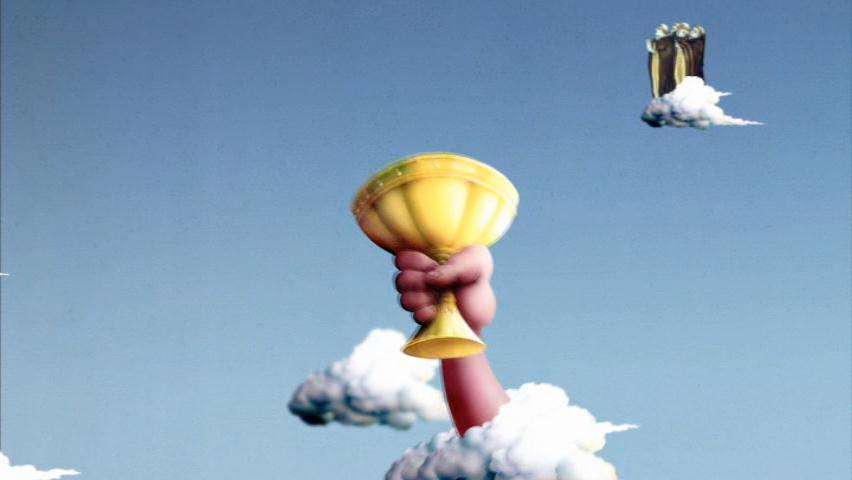
\includegraphics[width=0.8\textwidth]{grail.jpg}
    \caption[Voorbeeld figuur.]{\label{fig:grail}Voorbeeld van invoegen van een figuur. Zorg altijd voor een uitgebreid bijschrift dat de figuur volledig beschrijft zonder in de tekst te moeten gaan zoeken. Vergeet ook je bronvermelding niet!}
\end{figure}